\documentclass[a4paper,11pt]{article}
\usepackage[ngerman]{babel}
\usepackage[utf8]{inputenc}
\usepackage{amsmath}
\usepackage{graphicx} 
\title{Kartendarstellungen mit\newline matplotlib Toolkit basemap}
\author{Simon von Hall}
%\date{}


\begin{document}
\maketitle
\clearpage
\section{Eidesstattliche Erklärung}
Hiermit versichere ich, dass ich die Seminararbeit mit dem Thema Kartendarstellungen mit  \textsf{matplotlib Toolkit basemap} selbstständig verfasst und keine anderen als die angegebenen Quellen und Hilfsmittel benutzt habe, alle Ausführungen, die anderen Schriften
wörtlich oder sinngemäß entnommen wurden, kenntlich gemacht sind und
die Arbeit in gleicher oder ähnlicher Fassung noch nicht Bestandteil einer
Studien- oder Prüfungsleistung war.\\

Name: Simon von Hall\\

Jülich, den 15.12.14\\

Unterschrift des Studenten
\clearpage
\tableofcontents
\clearpage
\section{Vorwort}
\label{sec:vor}
In dieser Seminararbeit möchte ich das Python Modul \textsf{Basemap} vorstellen. Dazu werde ich die verschiedenen Kartenprojektionen die es unterstützt kurz beschreiben. Danach gehe ich auf die Funktionen des Moduls ein und beschreibe, was diese machen. Dabei gehe ich dann noch ganz kurz darauf ein, was für Voraussetzungen das Modul erwartet. Ich erkläre außerdem, wie man einfach mit dem Koordinatensystem umgehen kann. Zum Schluss erkläre ich noch, wie man die Karten, die man erstellt hat speichert.
\section{Kartendarstellungen}
\label{sec:2}
In diesem Kapitel möchte ich die vom Modul \textsf{Basemap} unterstützten Kartenprojektionen kurz beschreiben.\\
 \subsection{Azimuthale äquidistante Projektion}
\label{sec:azimuequi}
Bei dieser Projektion ist die kürzeste Entfernung vom Mittelpunkt der Karte zu einem beliebigen anderen Punkt eine gerade Linie. Das bedeutet, dass alle Punkte, die auf einem Kreis um den Kartenmittelpunkt liegen, äquidistant sind.\\
Nachteil:\newline
Die Gebiete die auf der anderen Seite der Welt liegen, werden sehr verzehrt dargestellt. Daher ist diese Projektion für Weltkarten 
eher ungeeignet.\\
\begin{figure}[hbtp]
\centering
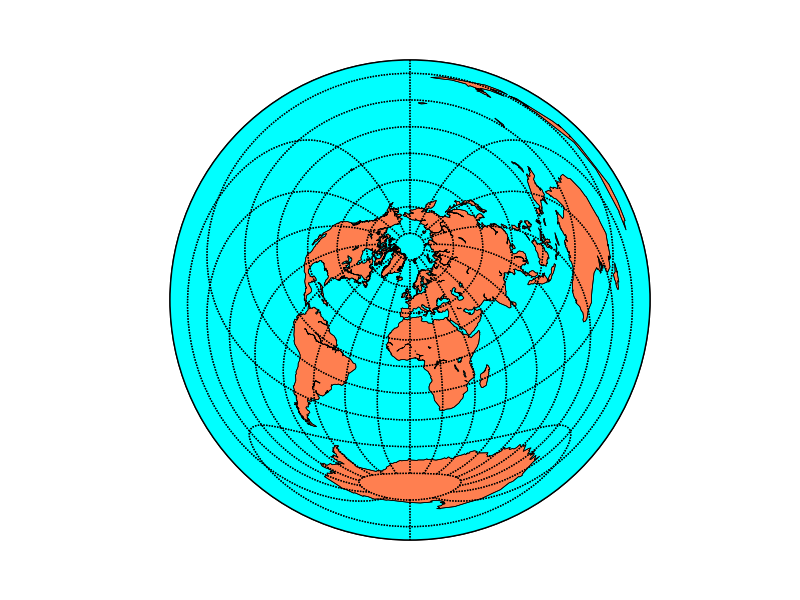
\includegraphics[scale=0.4,origin=c]{/Users/student/seminar/Kartendarstellungen/seminar/aziequi} \\
\caption{Azimuthale äquidistante Projektion}
\end{figure}
\clearpage
\subsection{Gnomonische Projektion}
\label{sec:gnomic}
In der gnomonischen Projektion werden alle Längenkreise als gerade Linien dargestellt.
Das Besondere der gnomonischen Projektion ist das der Projektionspunkt im Mittelpunkt der Erde liegt.
Da hier von Innen nach Außen projiziert wird, nimmt die Verzerrung mit der Entfernung vom Kartenmittelpunkt zu. Die gnomonische Projektion ist keine globale Projektion.\\

\begin{figure}[hbtp]
\centering
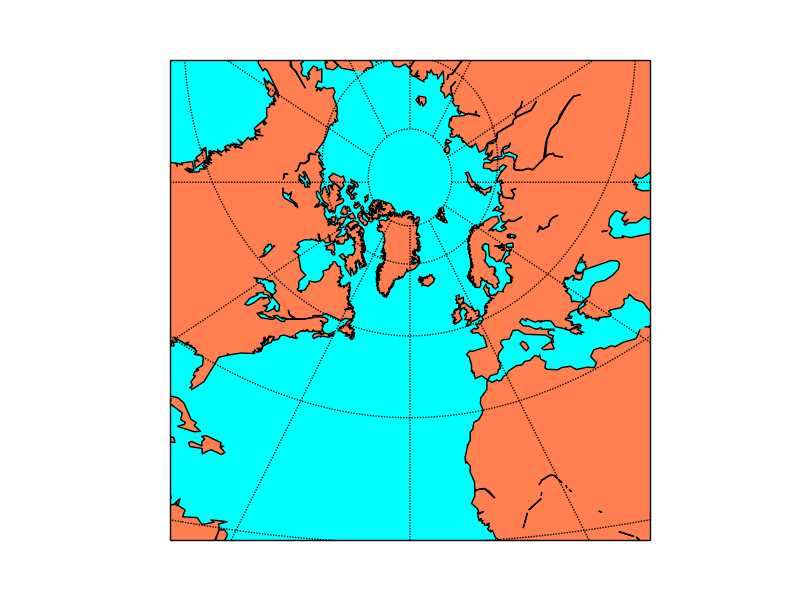
\includegraphics[scale=0.5,origin=c]{/Users/student/seminar/Kartendarstellungen/seminar/gnom} \caption{Gnomonische Projektion}
\end{figure}
\newpage 
\subsection{Orthographic Projection}
\label{sec:2.3}

\subsection{Geostationäre Projektion}
\label{sec:geostat}
In der geostationären Projektion wird die Erde aus der Perspektive eines geostationären Satelliten.
Vorteil:\newline \begin{itemize}
                  \item Wenn die Position des Satelliten bekannt ist, kann man dessen
                  Bilder als Hintergrund verwenden (siehe \ref{bilder})
                 \end{itemize}

Nachteil:\newline \begin{itemize}
                  \item Die andere Seite der Erde wird nicht dargestellt.\\
                  \item Entfernungen zwischen 2 Punkten werden auf Kreisbögen gemessen.\\
                  \item Der Satellit muss über dem Äquator sein.
                 \end{itemize}
\begin{figure}[hbtp]
\centering
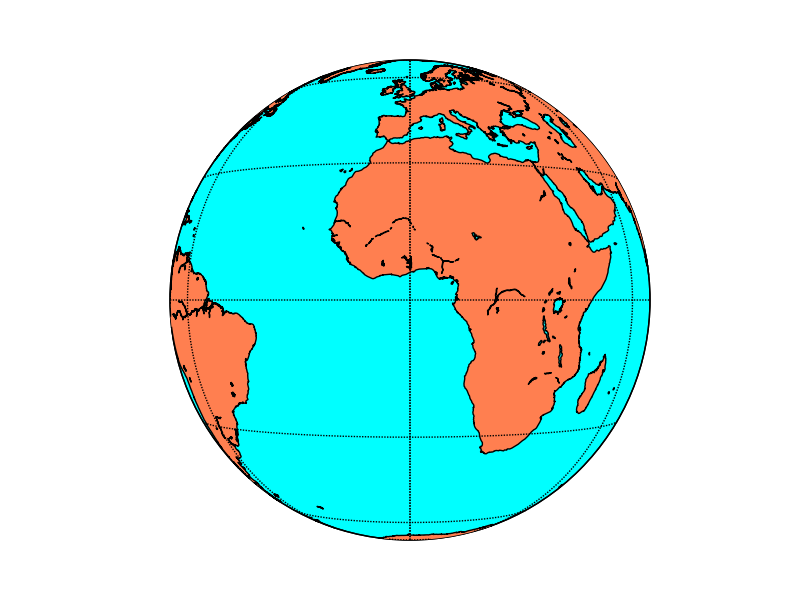
\includegraphics[scale=0.5,origin=c]{/Users/student/seminar/Kartendarstellungen/seminar/geos} \caption{Geostationäre Projektion}
\end{figure}
\newpage 
\subsection{Near-Sided perspektivische Projektion}
\label{sec:nearsideperspective}
Die Near Sided Perspective zeigt die Erde aus der Sicht eines Satelliten. Also ist es im Prinzip das selbe
wie die geostationäre Projektion.
\subsection{Mollweide Projection}
\label{sec:Mollweiden}
Bei der Mollweiden Projektion wird die Erde als Oval dargestellt. Die Mollweiden Projektion ist flächentreu.
Der Äquator und der Nullmeridian werden bei der Mollweiden Projektion maßstabsgetreu wieder gegeben.
Breitenkreise werden bei der Mollweiden Projektion als Geraden dargestellt. Die Längenkreise sind als Ellipsen dargestellt.
\subsection{Hammer Projektion}
\label{sec:Hammer}
Die Hammer Projektion ist wie die Mollweiden Projektion eine flächentreue Projektion.
Bei der Hammer Projektion wird die Erden ebenfalls als Oval dargestellt. Allerdings werden die Breitenkreise im Gegensatz zur Mollweiden Projektion als Ellipsen dargestellt, dadurch ist die Verzerrung an den Rändern nicht so stark. Nachteil bei dieser Art der Darstellung ist, dass die Erde an den Polen gestaucht wird.
\subsection{Robinson Projektion}
\label{sec:robinson}
Die Robinson Projektion ist eine globale Projektion. Die Erde wird hier annähernd Oval dargestellt. Die Pole werden allerdings in dieser Darstellung nicht abgedeckt. Breitenkreise werden in der Robinson Projektion als Geraden dargestellt. Bei dieser Darstellung wurden die Verzerrungen reduziert. Nachteil der Robinson Projektion ist das die Pole nicht erfasst werden.\\

\begin{figure}[hbtp]
\centering
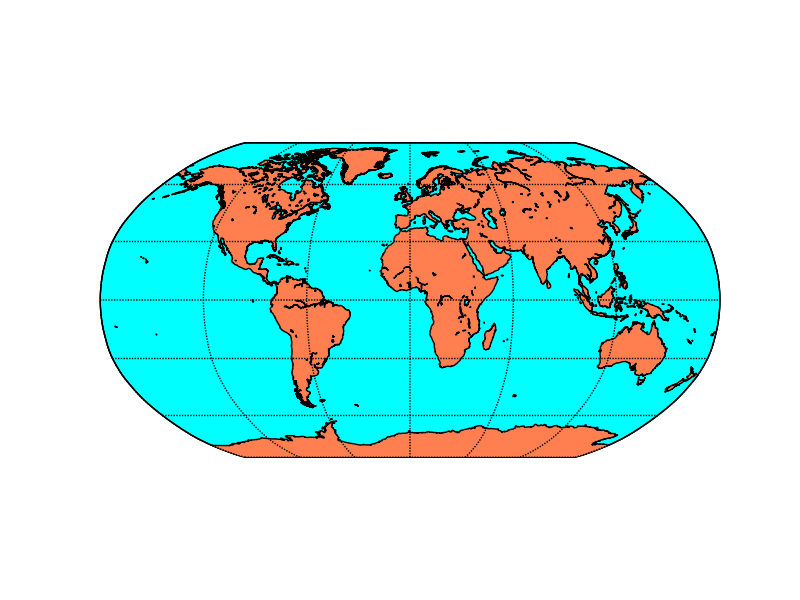
\includegraphics[scale=0.5,origin=c]{/Users/student/seminar/Kartendarstellungen/seminar/robin} \caption{Robinson Projektion}
\end{figure}
\newpage 
\subsection{Eckert 4 Projektion}
\label{sec:eckert4}
Die Eckert 4 Projektion ist sehr ähnlich wie die Robinson Projektion, allerdings ist Sie flächentreu. Deshalb ist die Darstellung an den Polen gestaucht. Die Erde wird wie auf einem Reifen dargestellt. Die Seitenränder sind in dieser Projektion Halbkreise.\newline
Formel:\newline

\begin{eqnarray*}
\mathcal{X}  & = & \frac{2}{\sqrt{4\pi +\pi ^2}}{\cal R}(\lambda -\lambda _0\footnote{Der zentrale Längenkreis} ) (1+\cos \theta)\\
\mathcal{Y}  & = & 2\sqrt{\dfrac{\pi }{4+\pi }}\cal R \sin \theta \\
\theta +\sin \theta \cos \theta +2\sin \theta & = &\left( 2+\frac{\pi }{2} \right) \sin \varphi
\end{eqnarray*}

\begin{figure}[hbtp]
\centering
 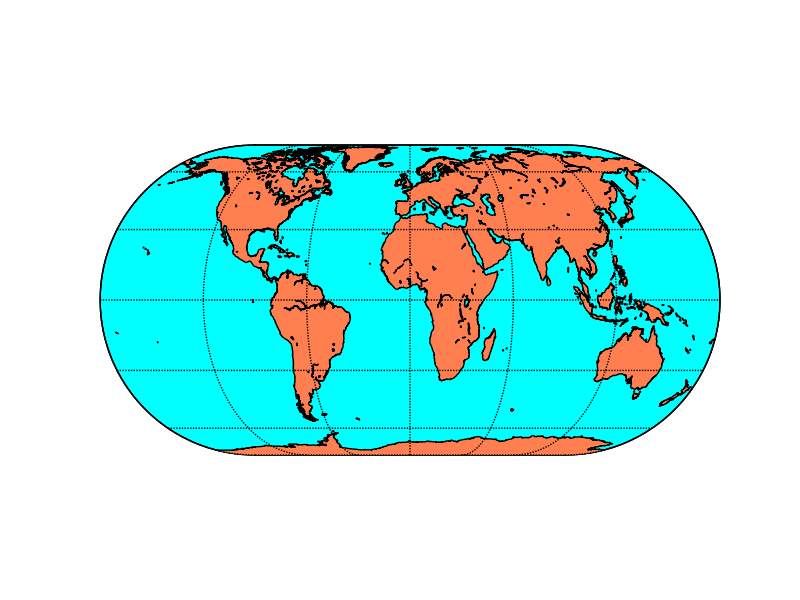
\includegraphics[scale=0.5,origin=c]{/Users/student/seminar/Kartendarstellungen/seminar/eck4} 
\caption{Eckert 4 Projektion}
\end{figure}
\newpage 
\subsection{Kavrayskiy 7 Projektion}
\label{sec:kravrayskiy}
Die Kavrayskiy 7 Projektion ist der Robinson Projektion sehr ähnlich. Sie stellt die Erde wieder annähernd oval dar. Die Breitenkreise werden in dieser Projektion als Geraden dargestellt. Diese Projektion stellt einen Kompromiss zwischen winkeltreuen und flächentreuen Projektionen dar.
\subsection{McBryde-Thomas Projektion}
\label{sec:mcbryde-thomas}
Diese Projektion ist eine flächentreue Darstellung der Erde. Die Breitenkreise werden als Geraden dargestellt. Die Längenkreise werden als Bögen dargestellt. Dabei haben die Längenkreise, auf einem Breitenkreis, immer den gleichen Abstand zueinander. Die Breitenkreise hingegen stehen immer näher je näher man den Polen kommt. Die Pole sind auf ein drittel des Äquators gestreckt. Der Nullmeridian ist in dieser Projektion 0,45 mal so lang wie der Äquator.

%Grapfik
\subsection{Sinusoidale Projektion}
\label{sec:sinusodial}
Die sinusoidale Projektion ist eine flächentreue Projektion. Auch in dieser Projektion werden die Breitenkreise als Geraden dargestellt. Das besondere an der sinusoidalen Projektion ist das die Länge der Breitenkreise relational zu $\cos\varphi$ ist, dies führt zu einer starken Verzerrung außerhalb der Mitte.\\
Vorteil der sinusoidalen Projektion:\\
\begin{itemize}
\item Die Projektion ist einfach zu berechnen.
\end{itemize}
Nachteil der sinusoidalen Projektion:\\
\begin{itemize}
\item Die Projektion ist nicht sehr anschaulich.
\end{itemize}
Formel:\\
\begin{eqnarray}
\mathcal {X} & = &\cal{R}\cdot(\lambda - \lambda _0)\cdot \cos \varphi \\
\mathcal{Y} & = &\cal{R} \cdot \varphi
\end{eqnarray}

\subsection{Äquidistante Zylinder Projektion}
\label{sec:aequizylinder} 
Die äquidistante Zylinder Projektion ist die einfachste Projektion. Sie stellt die Erde einfach in Längen- und Breitengrad dar. Dabei entsteht ein gleichmäßiges Gitterraster. Die Projektion ist weder winkel- noch flächentreu, das heißt, dass die Verzerrung mit der Entfernung vom Mittelpunkt der Karte zunimmt.\\ 
Vorteil der äquidistanten Zylinder Projektion:
\begin{itemize}
\item Die Projektion ist sehr einfach zu berechnen.
\end{itemize}
Nachteil der äquidistanten Zylinder Projektion:\\
\begin{itemize}
\item Die Verzerrungen wirken sowohl auf die Fläche als auch auf die Abstände aus.
\end{itemize}

Formel:\\
\begin{eqnarray}
\cal{X} & = & \lambda\\
\cal{Y} & = & \varphi
\end{eqnarray}
\subsection{Cassini Projektion}
\label{sec:cassini}
Bei der Cassini Projektion wird die Erde zuerst gedreht, sodass der Äquator zum Nullmeridian wird.
Danach wird dann eine äquidistante Zylinder Projektion angewendet. \\

\begin{figure}[hbtp]
\centering
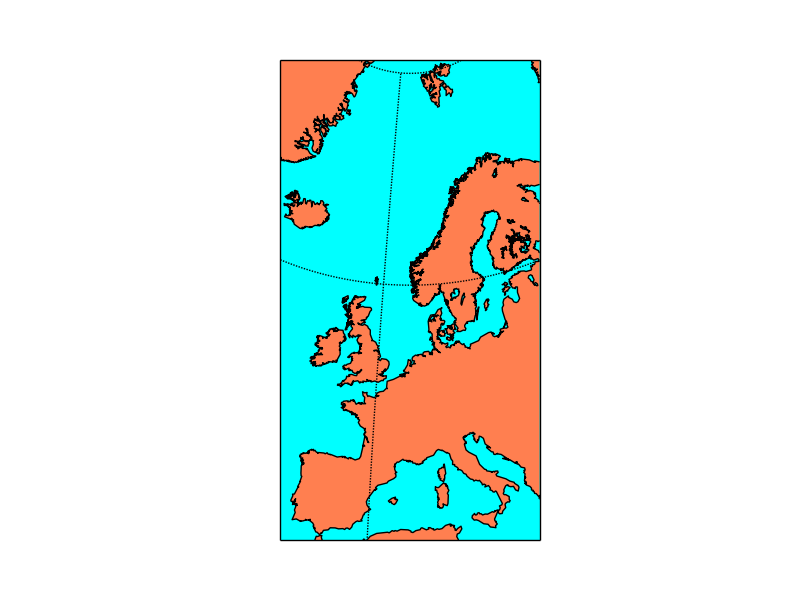
\includegraphics[scale=0.5,origin=c]{/Users/student/seminar/Kartendarstellungen/seminar/cass} \caption{Cassini Projektion}
\end{figure}
\newpage 
\subsection{Mercatorprojektion}
\label{sec:mercator} 
Die Mercatorprojektion ist eine winkeltreue Zylinderprojektion. Sie erreicht dabei nie Pole.
Die Längengrade verlaufen in dieser Projektion parallel und haben den gleichen Abstand zueinander.
Die Breitengrade sind ebenfalls parallel zueinander haben aber unterschiedliche Abstände.
Die Verzerrung nimmt mit Polnähe zu, das heißt, dass die Karte zu den Polen hin gestreckt wird.\\

\begin{figure}[hbtp]
\centering
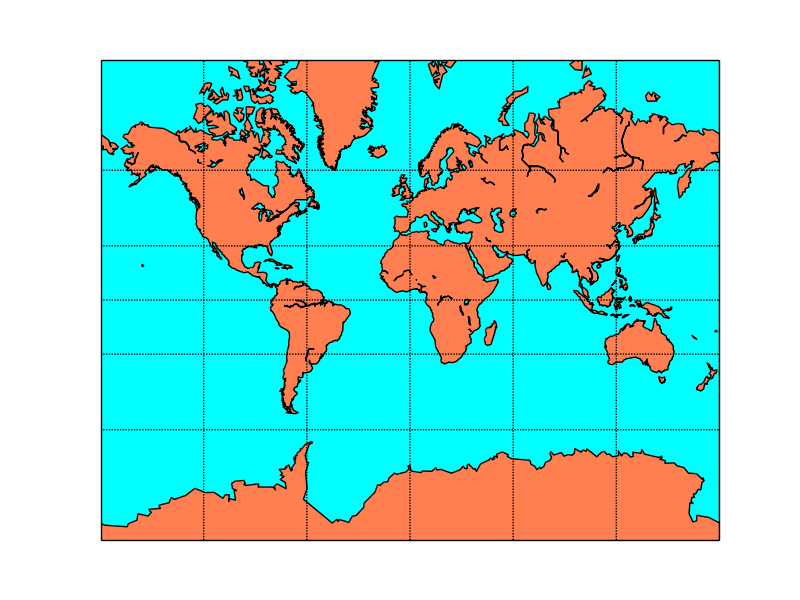
\includegraphics[scale=0.5,origin=c]{/Users/student/seminar/Kartendarstellungen/seminar/merc} \caption{Mercatorprojektion}
\end{figure}
\newpage 
\subsection{Transversale Mercatorprojektion}
\label{sec:transmercator}
Bei der transversalen  Mercatorprojektion wird der Globus zuerst um 90° gedreht, so das der 0 Meridian zu Äquator wird. Danach wird eine normale Mercatorprojektion erstellt.
\subsection{Schiefe Mercatorprojektion}
\label{sec:schiefmerc}
Bei der schiefen Mercatorprojektion kann die zentrale Linie jede Linie zwischen zwei Punkten sein und nicht wie bei der Mercatorprojektion nur ein Breitengrad oder der transversen Mercatorprojektion nur ein Längengrad.
\subsection{Polykonische Projektion}
\label{sec:polikonisch}
Die polikonische Projektion ist eine globale Projektion. Hierbei werden auf dem zentralen Meridian unendlich viele Kegel aufgebaut. Dabei entstehen nicht konzentrische Breitenkreise. Die Projektion geht an den Polen auseinander. Die Verzerrung der Fläche nimmt mit der Entfernung vom zentralen Meridian der Karte zu. Die Winkel sind lokal entlang des zentralen Längengrades genau, sonst sind sie verzerrt.
\subsection{Miller Zylinderprojektion}
\label{sec:miller}
Die Miller Zylinderprojektion ist eine globale Projektion. Sie ist der Mercatorprojektion sehr ähnlich.
Allerdings ist hier die Verzerrung an den Polen anders. Die Pole werden nicht mehr so stark gesteckt, dafür ist die Miller-Projektion nicht winkeltreu. Dafür reicht die Miller Zylinderprojektion bis an die Pole. \\

\begin{figure}[hbtp]
\centering
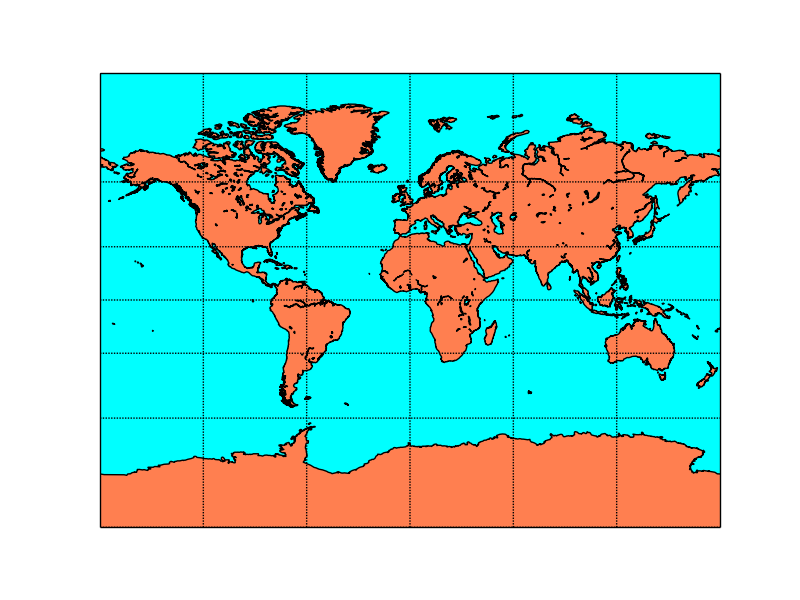
\includegraphics[scale=0.5,origin=c]{/Users/student/seminar/Kartendarstellungen/seminar/mill} \caption{Miller Zylinderprojektion}
\end{figure}
\newpage 
\subsection{Stereographische Gall Projektion}
\label{sec:stereogall} 
Die stereographische Gall Projektion ist eine globale Zylinderprojektion. Die Gall Projektion hat zwei Standartparallelen bei 45$ ^\circ $N und 45$^\circ $S. Die Verzerrung der Fläche und Winkel nimmt mit Abstand zu den Standartparallelen zu. Die Verzerrung ist allgemein an den Polen sehr stark. \\

\begin{figure}[hbtp]
\centering
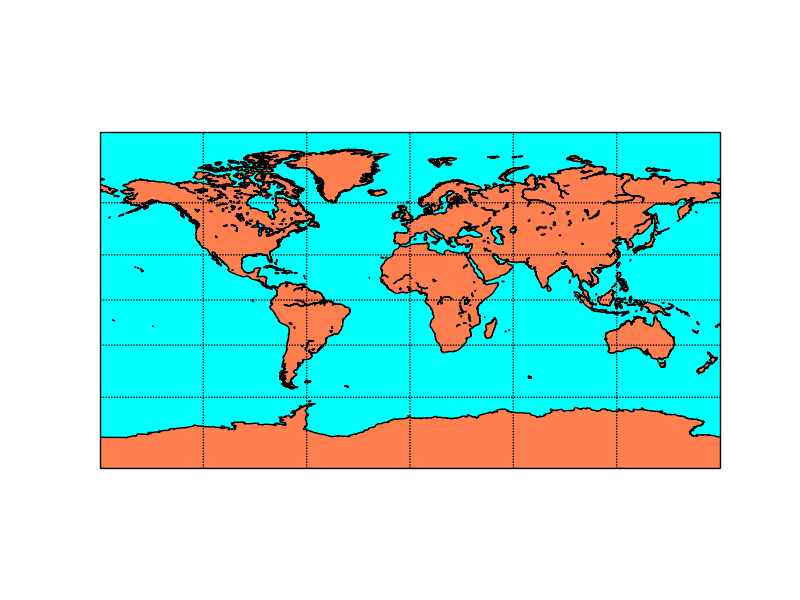
\includegraphics[scale=0.5,origin=c]{/Users/student/seminar/Kartendarstellungen/seminar/gall} \caption{Stereographische Gall Projektion}
\end{figure}
\newpage 
\subsection{Flächentreue Zylinderprojektion}
\label{sec:equareazyl}
Die flächentreue Zylinderprojektion ist eine flächentreue Zylinderprojektion wie es der Name bereits sagt. 
\subsection{ Winkeltreue Lambert Projektion}
\label{sec:lamwink}
Die winkeltreue Lambert Projektion ist winkeltreu. Die Längenkreise werden als Geraden dargestellt.
Die winkeltreue Lambert Projektion ist eine Kegelprojektion. 

Formel:\\
 \begin{eqnarray*}
 \mathcal{X}& = &\rho \sin ( n(\lambda -\lambda _0) )\\
 \mathcal{Y}& = &\rho _0-\rho \cos (n(\lambda - \lambda _0))\\
 \rho & = &F\cot ^n(\frac{1}{4}\pi + \frac{1}{2}\varphi)\\
 n& = &\dfrac{\ln (\cos \varphi _1 \sec \varphi _2)}{\ln (\tan (\frac{1}{4}\pi +\frac{1}{2}\varphi _2)\cot (\frac{1}{4}\pi + \frac{1}{2}\varphi _1))}\\
 F& = &\dfrac{\cos \varphi _1 \tan ^n(\frac{1}{4}\pi +\frac{1}{2}\varphi _1)}{n}
 \end{eqnarray*}\\
 
\begin{figure}[hbtp]
\centering
 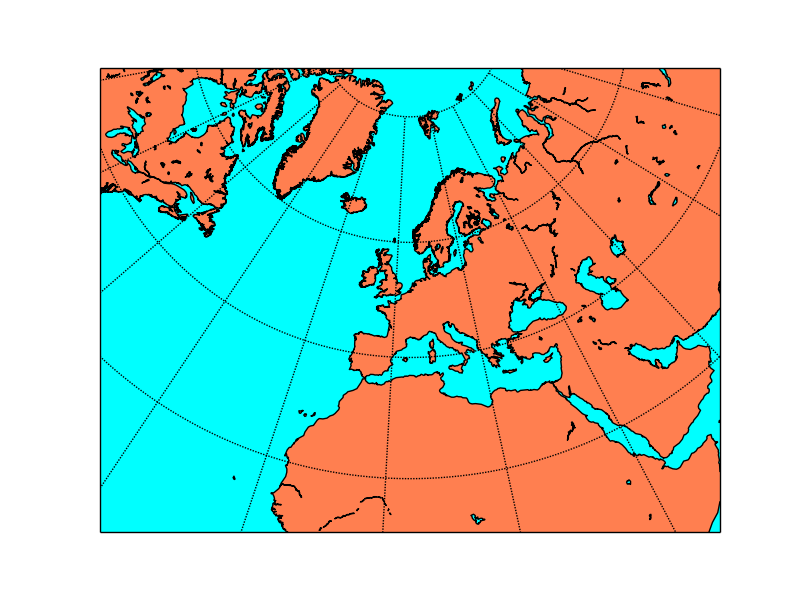
\includegraphics[scale=0.5,origin=c]{/Users/student/seminar/Kartendarstellungen/seminar/lcc} \caption{Winkeltreue Lambert-Projektion}
\end{figure}
\newpage 
\subsection{Azimuthale Flächentreue Lambert-Projektion}
\label{sec:lamflach}
\subsection{Stereografische Projektion}
\label{sec:stereo}
Die stereografische Projektion ist eine winkeltreue Projektion. Sie ist allerdings nicht flächentreu.
Man kann mit dieser Projektion die ganze Erde abbilden allerdings nimmt die Verzerrung sehr schnell stark zu, weshalb die stereografische Projektion  für globale Abbildungen eher ungeeignet ist. Diese Projektion erhält man, wenn man von einem Ausgangspunkt geraden durch jeden Punkt der Erde zieht, die Schnittpunkte dieser Geraden mit der Projektionsebene sind die Punkte auf die projiziert wird.
Die Projektionsebene kann grundsätzlich frei positioniert werden.\\

\begin{figure}[hbtp]
\centering
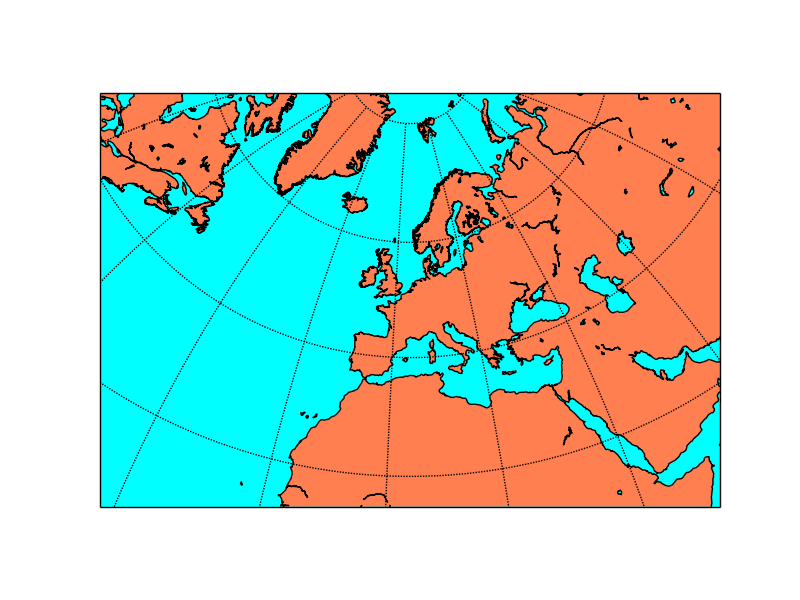
\includegraphics[scale=0.5,origin=c]{/Users/student/seminar/Kartendarstellungen/seminar/stere} \caption{Stereografische Projektion}
\end{figure}
\newpage 
\subsection{Längentreue Kegelprojektion}
\label{sec:langkeg}
Die längentreue Kegelprojektion ist eine globale Projektion. Sie ist weder winkel- noch flächentreu.
Die Verzerrung nimmt zum Kartenrand hin zu. Die Breitenkreise sind in dieser Projektion gleichmäßig verteilt, und die Längenkreise werden als Geraden dargestellt. Die Projektion bildet die Erde auf einen Kegelmantel ab.
\subsection{Flächentreue Albert-Projektion}
\label{sec:albert}
Die flächentreue Albert-Projektion ist eine globale Kegelprojektion. Sie bildet die Erde auf einen Kegelmantel ab. Sie benutzt für die Projektion 2 Standardbreitenkreise. 
\\

Formel:\\ 
\begin{eqnarray*}
\mathcal{X}&=&\rho \sin \theta \\
\mathcal{Y}&=&\rho _0 -\rho \cos \theta\\
\\
n&=&\frac{1}{2}(\sin \varphi _1 +\sin \varphi _2)\\
\theta &=&n(\lambda -\lambda _0)\\
\tau &=&\cos ^2 \varphi _1 +2n\sin \varphi _1\\
\rho &=&\dfrac{\sqrt{\tau -2n\sin \varphi}}{n}\\
\rho _0 &=&\dfrac{\sqrt{\tau -2n\sin \varphi _0}}{n}
\end{eqnarray*}

\begin{figure}[hbtp]
\centering
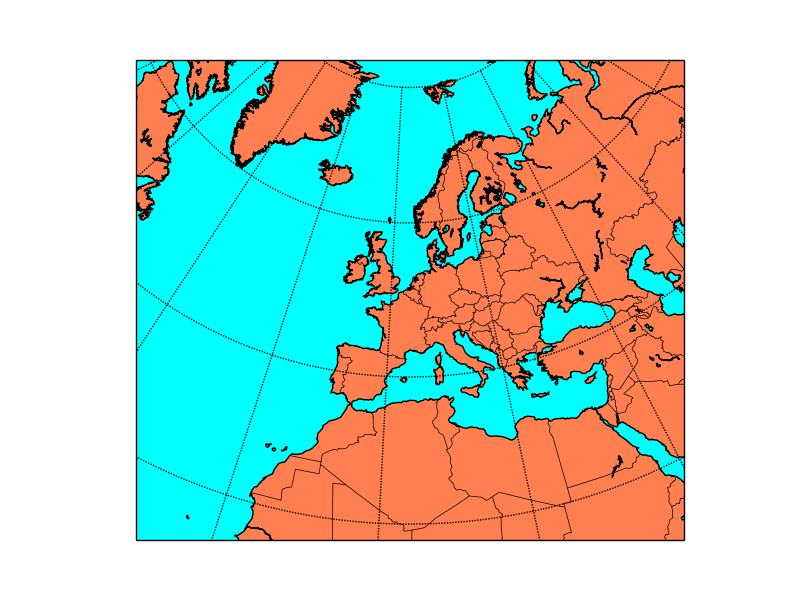
\includegraphics[scale=0.5,origin=c]{/Users/student/seminar/Kartendarstellungen/seminar/aea} \\
\caption{Flächentreue Albert-Projektion}
\end{figure}
\newpage 
\subsection{Polare stereographische Projektion}
\label{sec:polstere}
Die polare stereographische  Projektion ist eine stereographische Projektion die einen der beiden Pole als Kartenzentrum hat.\\
\subsection{Polare azimutale Lambertprojektion}
\label{sec:pollam}
Die polare  azimutale Lambertprojektion hat ebenfalls einfach nur einen Pol als Kartenzentrum.
\subsection{Polare azimuthale äquidistante Projektion}
\label{sec:polaequi}
Diese Projektion hat ebenfalls einfach einen Pol als Mittelpunkt. 
\subsection{Van der Grinten Projektion}
\label{sec:vander}
Die van der Grinten Projektion ist eine globale Projektion, die die Erde auf einen Kreis projiziert. Diese Projektion ist weder winkel- noch flächentreu. Die Verzerrung nimmt zum Rand hin zu. Die van der Grinten Projektion ist um den Äquator zentriert.\\
Formel:\\
\begin{eqnarray*}
\mathcal{X}&=&\dfrac{\pm \pi(A(G-P^2)+\sqrt{A^2(G-P^2)^2 -(A^2 +P^2)(G^2 -P^2)})}{P^2 +A^2}\\
\mathcal{Y}&=&\dfrac{\pm \pi (PQ-A\sqrt{(A^2 +1)(P^2 +A^2)-Q^2})}{P^2 +A^2}\\
\\
A&=&\frac{1}{2}\vert \dfrac{\pi}{\lambda -\lambda _0}-\dfrac{\lambda -\lambda _0}{\pi}\vert\\
G&=&\dfrac{\cos \theta}{\sin \theta +\cos \theta -1}\\
P&=&G(\dfrac{2}{\sin\theta}-1)\\
\theta &=&\arcsin \vert\dfrac{2\varphi}{\pi}\vert\\
Q&=&A^2 +G\\
 &Falls \varphi =0:\\
 \mathcal{X}&=&\lambda -\lambda _0\\
 \mathcal{Y}&=&0\\
 &Falls \lambda =\lambda _0 oder \varphi =\pm\frac{\pi}{2}:\\
 \mathcal{X}&=&0\\
 \mathcal{Y}&=&\pm \pi \tan \frac{\theta}{2}
\end{eqnarray*}

\begin{figure}[hbtp]
\centering
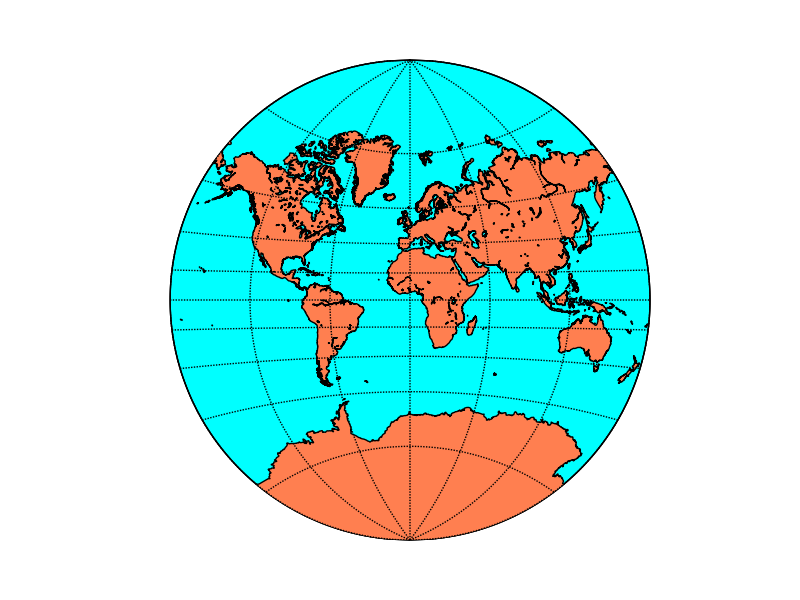
\includegraphics[scale=0.5,origin=c]{/Users/student/seminar/Kartendarstellungen/seminar/vandg} \caption{Van der Grinten Projektion}
\end{figure}
\newpage 
\newpage
\section{Basemap}
\subsection{Einführung}
Das Toolkit Basemap ist ein Pythonmodul zur bearbeitumg von Karten.
Es bietet viele verschiedene Arten Karten in 2D darzustellen (siehe Projektionen \ref{Projektionen} )
Es ermöglicht einem auch das Ploten auf den Karten. Hierbei kann man, dann auch Längen- und Breitengrad
als Positionsangabe nutzen. Das Basemap Toolkit wandelt die Koordinaten dann mit der PROJ4 Library in 
die entsprechenden 2D Koordinaten um.
\subsection[Dependencies]{Abhängigkeiten voon basemap}
Das Toolkit setzt folgende Voraussetzungen:
\newline
\begin{itemize}
 \item Python
 \item Numpy
 \item Matplotlib
 \item GEOSlib (ist im Projekt enthalten)
 \item PROJ4 (ist im Projekt enthalten)
 \item dateutil
 \item pyparsing
 \item six
 \item libpng
 \\
 \item PIL (ist optional)\\
 PIL wird nur gebraucht um auf mehr Bildformate zugreifen zu können.
 \item 
\end{itemize}

\subsection{Erstellen einer Karte mit Basemap}
\label{sec:erstellen}
Eine Karte erzeugt man mit der Klasse \emph{Basemap}. Die Funktion ist wie folgt definiert:
\begin{verse}
\textsf{ Basemap(llcrnrlon=None, llcrnrlat=None, urcrnrlon=None, urcrnrlat=None, llcrnrx=None, llcrnry=None, urcrnrx=None, urcrnry=None, width=None, height=None, projection='cyl', resolution='c', area\_thresh=None, rsphere=6370997.0, ellps=None, lat\_ts=None, lat\_1=None, lat\_2=None, lat\_0=None, lon\_0=None, lon\_1=None, lon\_2=None, o\_lon\_p=None, o\_lat\_p=None, k\_0=None, no\_rot=False, suppress\_ticks=True, satellite\_height=35786000, boundinglat=None, fix\_aspect=True, anchor='C', celestial=False, round=False, epsg=None, ax=None)
}\end{verse}
Dabei kann der Parameter \textsf{projection} folgende Werte haben:
\newline
\begin{tabular}{r@{ }l}
cea &	Cylindrical Equal Area\\
mbtfpq &	McBryde-Thomas Flat-Polar Quartic\\
aeqd &	Azimuthal Equidistant\\
sinu &	Sinusoidal\\
poly &	Polyconic\\
omerc &	Oblique Mercator\\
gnom &	Gnomonic\\
moll &	Mollweide\\
lcc &	Lambert Conformal\\
tmerc &	Transverse Mercator\\
nplaea &	North-Polar Lambert Azimuthal\\
gall &	Gall Stereographic Cylindrical\\
npaeqd &	North-Polar Azimuthal Equidistant\\
mill &	Miller Cylindrical\\
merc &	Mercator\\
stere &	Stereographic\\
eqdc &	Equidistant Conic\\
rotpole &	Rotated Pole\\
cyl &	Cylindrical Equidistant\\
npstere &	North-Polar Stereographic\\
spstere &	South-Polar Stereographic\\
hammer &	Hammer\\
geos &	Geostationary\\
nsper &	Near-Sided Perspective\\
eck4 &	Eckert IV\\
aea &	Albers Equal Area\\
kav7 &	Kavrayskiy VII\\
spaeqd &	South-Polar Azimuthal Equidistant\\
npaepd & North-Polar Azimuthal Equidistant\\
ortho &	Orthographic\\
cass &	Cassini-Soldner\\
vandg& 	van der Grinten\\
laea &	Lambert Azimuthal Equal Area\\
splaea &	South-Polar Lambert Azimuthal\\
nplaea & North-Polar Lambert Azimuthal\\
robin &	Robinson
\end{tabular}

Die Parameter \textsf{width, height} geben die Breite, beziehungsweise die Höhe der Karte in Metern an,
diese Parameter können bei den folgenden Projektionen nicht gesetzt werden.
\begin{verse}
\textsf{sinu, moll, hammer, npstere, spstere, nplaea, splaea, npaepd, spaepd, robin, eck4, kav7, mbtfpq, ortho, geos, nsper}
\end{verse}
Die Parameter \textsf{lon\_0 ,lat\_0 } nehmen die Koordinate des Kartenmittelpunkts in Grad, beziehungsweise den zentralen Längen- oder Breitengrad.\\
Die Parameter \textsf{urcrnrlon, urcrnrlat, llcrnrlon, llcrnrlat, urcrnrx, urcrnry, llcrnrx, llcrnry} sind die Koordinaten der untere linke und oberen rechten Ecke der Karte, in Grad oder Meter mit (0,0) im Mittelpunkt der Karte. Eine der beiden Arten die Grenzen der Karte festzulegen muss angegeben werden außer bei den folgenden Projektionen:\\
\begin{verse}
\textsf{sinu, moll, hammer, npstere, spstere, nplaea, splaea, npaepd, spaepd, robin, eck4, kav7, mbtfpq}
\end{verse}
Da diese entweder immer den ganzen Globus zeigen oder die Grenzen automatisch ermittelt werden.
Bei der \textsf{rotpole} Projektion werden mit lat/lon die Ecken des nicht rotierten Globus angegeben mit x/y die Ecken des rotierten Globus.
Bei dem Parameter \textsf{resolution} kann man die Werte \textsf{c, l, i, h, f, None} haben, falls \textsf{None} angegeben wurde, werden keine Grenzdaten geladen weshalb Klassenmethoden Fehler werfen.\\
 Der Parameter \textsf{area\_tresh} gibt an welche Mindest-Fläche Seen haben müssen um gezeichnet zu werden. Der Defaultwert ist 10000, 1000, 100, 10, 1 für die Resolution von c, l, i, h, f. Die Werte geben die Fläche in $km^2$.\\
 Der Parameter \textsf{rsphere} bekommt den Radius, der der Projektion zugrunde liegenden Figur, in Metern.
 Bei einer Kugel wird nur ein Wert angegeben, bei einem Ellipsoiden wird ein Array mit zwei Werten erwartet.\\
 Über den Parameter \textsf{ellps} kann man die Form der Erde mit Hilfe spezieller Zeichenketten angeben.
 Sollte \textsf{ellps} angegeben sei wird \textsf{rsphere} ignoriert.\\
 Mit dem Parameter \textsf{supress\_ticks} kann man steuern ob die Achsen automatisch beschriftet und aufgeteilt werden sollen.\\
  Der Parameter \textsf{fix\_aspect} passt die Seitenverhältnisse vom Plot den Seitenverhältnissen der Karte an.\\
  Der Parameter \textsf{anchor} gibt an wo die Karte im Gitter liegt, gültige Werte für diesen Parameter sind:\\
  \begin{verse}
  \textsf{C, SW, S, SE, E, NE, N, NW, W}
  \end{verse}
  Mit dem Parameter \textsf{celestial} kann man einstellen das eine astronomische Konvention bezüglich der Längengrade benutzt wird. Was bedeutet, dass negative Längengrade östlich des Nullmeridian liegen.
  Diese Einstellung impliziert das die Resolution auf \textsf{None} gesetzt ist.\\
  Mit dem \textsf{ax} Parameter kann man eine eigene Achseninstanz übergeben, wenn nichts übergeben wird, versucht \textsf{basemap} sich die aktuelle Achseninstanz mit Hilfe von \textsf{pyplot.gca()} zu holen. Falls man nicht \textsf{pyplot} importiert kann man auch jeder Klassenmethode die zeichnet eine Achseninstanz übergeben auf der gezeichnet wird. Wenn man allerdings hier die Achseninstanz übergibt werden alle Methoden auf dieser Achseninstanz ausgeführt.\\
  Mit dem \textsf{lat\_ts} Parameter wird der Breitengrad angegeben, der Maßstabs getreu wiedergegeben wird. Dieser Parameter ist optional und nur für die Projektionen \textsf{stere, cea, merc} von Belang.\\
  Mit den Parametern \textsf{lat\_1, lat\_2} werden die Breitengrade der 1. und 2. Standartparallele angegeben. Diese sind nur für die Projektionen \textsf{lcc, aea, eqdc} interessant.\\
  Mit den Parametern \textsf{lon\_1, lon\_2} werden die Breitengerade für die Punkte auf der Zentralen Linie der \textsf{omerc} Projektion angegeben.\\
  Der Parameter \textsf{k\_0} gibt den Skalierungsfaktor am Ursprung an, welcher nur von den Projektionen \textsf{tmerc, omerc, stere, lcc} genutzt wird.\\
  Mit dem Parameter \textsf{no\_rot} kann man bei der \textsf{omerc} Projektion einstellen ob die Koordinaten rotiert werden oder nicht.
  Die Parameter \textsf{o\_lat\_p, o\_lon\_p} geben die Position des rotierten Pols in Grad an, dies wird nur von der Projektion \textsf{rotpole} verarbeitet.\\
  Der Parameter \textsf{boundinglat} gibt an bis zu welchem Breitengrad die polare Karte reicht.\\
  Mit dem Parameter \textsf{round} kann man einstellen ob an dem Grenzbreitengrad bei polaren Karten abgeschnitten werden soll oder nicht. Dadurch kann man einstellen ob die Karte rund oder eckig ist.\\
  Mit dem Parameter \textsf{satellite\_height} gibt man die Höhe des Satelliten über dem Äquator an. 
  Dies ist nur für die Projektionen \textsf{geos, nsper} interessant.\\
  Mit dieser Funktion kann man eine Karteninstanz erstellen, allerdings ist noch nichts gezeichnet worden.
  Dafür müssen noch weitere Funktionen aufgerufen werden. Welche ich im nächsten Unterkapitel beschreibe.
\subsection{Zeichnen der Karte}
\label{sec:zeichnenkarte}
Die Karte zeichnet man mit verschiedenen Methoden der Karte.\\
\subsubsection*{Küstenlinie zeichnen}
Die Küstenlinie zeichnet man mit der Funktion \textsf{ drawcoastlines(linewidth=1.0, linestyle='solid', color='k', antialiased=1, ax=None, zorder=None)}, man kann mit den Parametern einstellen wie die Küstenlinie gezeichnet werden soll. Mit dem Parameter \textsf{zorder}kann man die Reihenfolge in der gezeichnet wird beeinflussen. Niedrige Werte im Parameter \textsf{zorder} werden zuerst gezeichnet.
Mit dem Parameter \textsf{ax} kann man eine Achseninstanz übergeben auf der gezeichnet werden soll, normalerweise wird die Achseninstanz der Karte genommen. Sollte keine Achseninstanz gefunden werden wird ein Fehler geworfen.\\
\lstinputlisting{/Users/student/seminar/bsp/bspcoast.py}
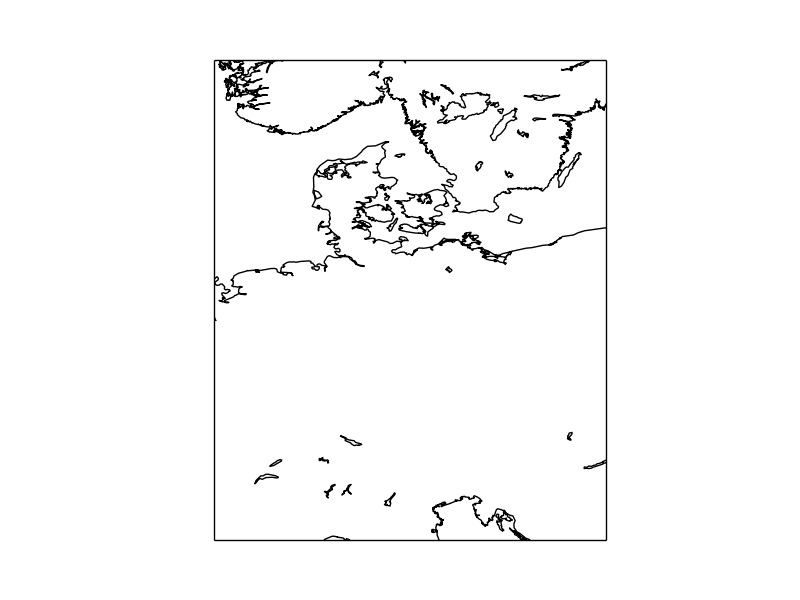
\includegraphics[scale=0.4]{/Users/student/seminar/bsp/bspcoast}\newpage 
\subsubsection*{Ländergrenzen zeichnen}
Ländergrenzen können mit der Funktion \textsf{ drawcountries(linewidth=0.5, linestyle='solid', color='k', antialiased=1, ax=None, zorder=None)} gezeichnet werden. Die Parameter sind die selben wie beim zeichnen der Küstenlinien. \\
Mit der Funktion \textsf{drawcounties(linewidth=0.1, linestyle='solid', color='k', antialiased=1, facecolor='none', ax=None, zorder=None, drawbounds=False)} können die Countiegrenzen in den USA gezeichnet werden. Mit dem Parameter \textsf{facecolor} kann eine Farbe angegeben werden mit der gefüllt werden soll.\\
Mit der Funktion \textsf{drawstates(linewidth=0.5, linestyle='solid', color='k', antialiased=1, ax=None, zorder=None)} können die Staatsgrenzen in den USA gezeichnet werden.\\
\lstinputlisting{/Users/student/seminar/bsp/bspland.py}
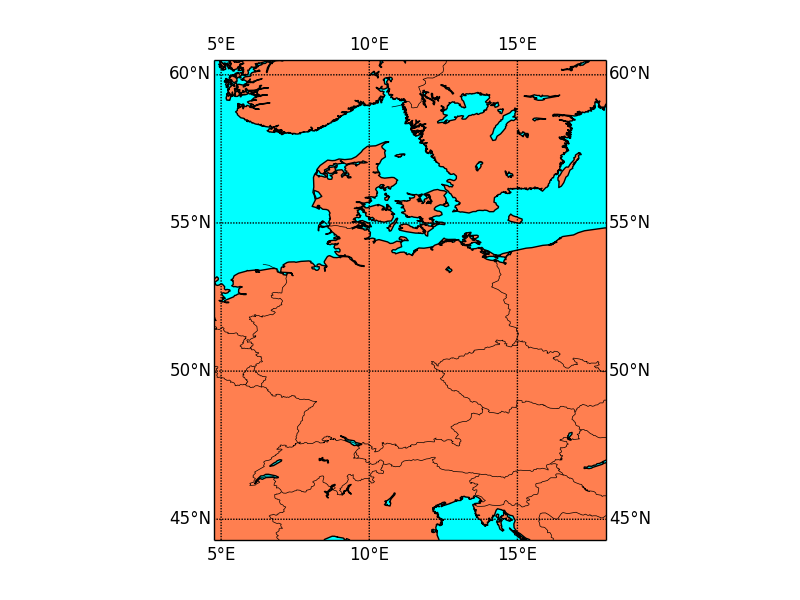
\includegraphics[scale=0.4]{/Users/student/seminar/bsp/bspland}\newpage 
 \subsubsection*{Fülle der Karte}
 Mit der Funktion \textsf{fillcontinents(color='0.8', lake\_color=None, ax=None, zorder=None, alpha=None)} kann man die Kontinente und Seen mit Farben füllen.
 Mit der Funktion \textsf{drawmapboundary(color='k', linewidth=1.0, fill\_color=None, zorder=None, ax=None)} kann man die Kartengrenze zeichnen und die Karte mit einer Farbe füllen. So kann man die Ozeane mit einer Farbe füllen, wenn man die Kontinente ebenfalls mit Farbe füllt. Sonst hat alles die gleiche Farbe.\\
 Man kann die Karte auch mit Hilfe der Funktion \textsf{drawlsmask(land\_color='0.8', ocean\_color='w', lsmask=None, lsmask\_lons=None, lsmask\_lats=None, lakes=True, resolution='l', grid=5, **kwargs)} füllen.
 Diese Funktion zeichnet ein Bild, daher kann man keine Zeichenreihenfolge angeben. Die Funktion erwartet im Parameter \textsf{lsmask} eine Matrix mit den Werten 0 für ein Ozean Pixel, 1 für ein Land Pixel und 2 für ein See Pixel. In den Parametern \textsf{lsmask\_lon} und \textsf{lsmask\_lat} erwartet die Funktion eindimensionale Arrays für die Längen- und Breitengrade der \textsf{lsmask}, sie müssen aufsteigend sortiert sein.\\
 \lstinputlisting{/Users/student/seminar/bsp/bspbase.py}
 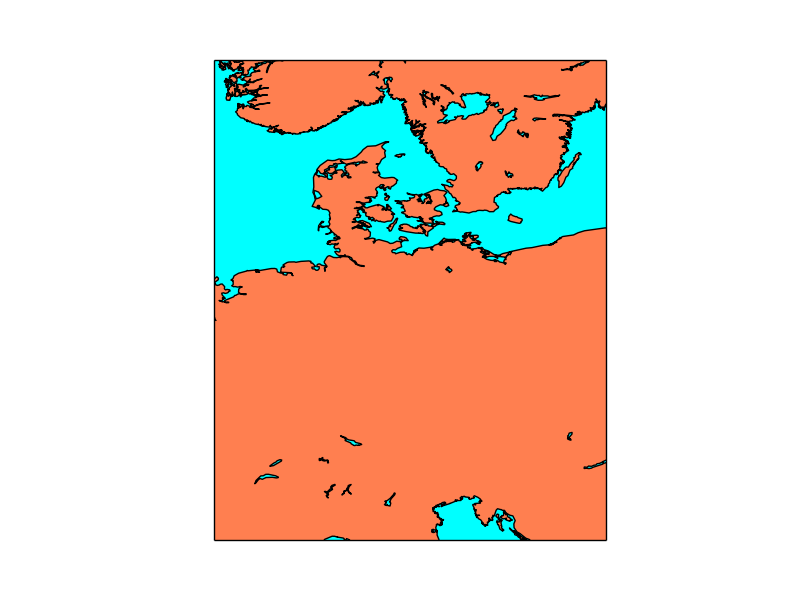
\includegraphics[scale=0.4]{/Users/student/seminar/bsp/bspbase}\newpage 
 \subsubsection*{Flüsse zeichnen}
 Die Funktion \textsf{drawrivers(linewidth=0.5, linestyle='solid', color='k', antialiased=1, ax=None, zorder=None)} ermöglicht es Flüsse zu zeichnen. Es sind allerdings nicht alle Flüsse erfasst. Die größeren sind allerdings erfasst.\\
 \lstinputlisting{/Users/student/seminar/bsp/bsprivers.py}
 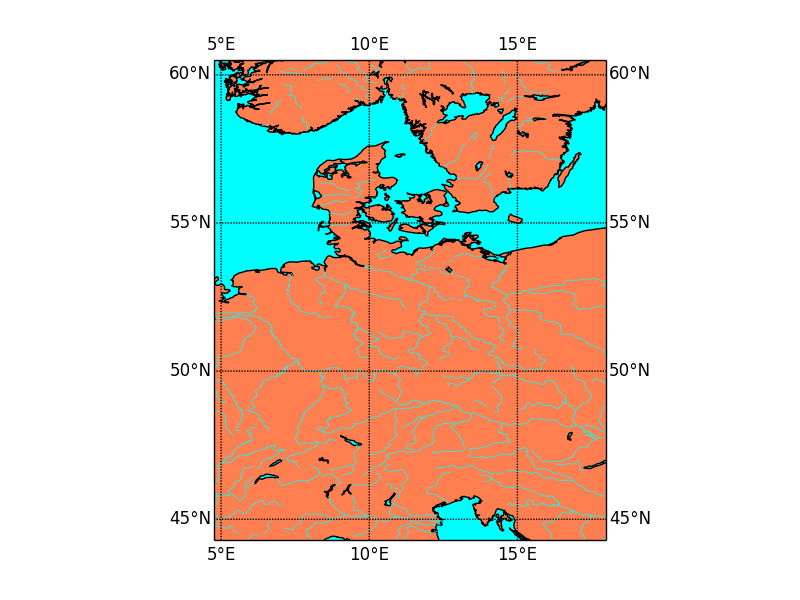
\includegraphics[scale=0.4]{/Users/student/seminar/bsp/bsprivers}\newpage 
 \subsubsection*{Längen- und Breitengrade zeichnen}
 Längen- und Breitengrade kann man einfach mit den Funktionen \textsf{drawmeridians(meridians, color='k', linewidth=1.0, zorder=None, dashes=[1, 1], labels=[0, 0, 0, 0], labelstyle=None, fmt='\%g', xoffset=None, yoffset=None, ax=None, latmax=None, **kwargs)} und \textsf{drawparallels(circles, color='k', linewidth=1.0, zorder=None, dashes=[1, 1], labels=[0, 0, 0, 0], labelstyle=None, fmt='\%g', xoffset=None, yoffset=None, ax=None, latmax=None, **kwargs)} zeichnen. Der Parameter \textsf{labels} gibt an wo die Grade beschriftet werden sollen links, rechts, oben, unten. Mit dem Parameter \textsf{labelstyle} kann man einstellen ob die Grade mit $ \pm $ oder mit E, W beziehungsweise N, S beschriftet werden sollen. Falls nichts angegeben wird, werden die Buchstaben benutzt. Dem Parameter \textsf{fmt} kann eine Funktion übergeben werden die aus dem Gradwert eine Zeichenkette macht.
 Mit dem Parameter \textsf{meridians} beziehungsweise \textsf{circles} wird eine Liste der Grade übergeben die gezeichnet werden sollen. Über den Parameter \textsf{dashes} kann man ein Pattern definieren mit dem die Grade gezeichnet werden sollen. Es werden immer abwechselnd die Anzahl an Pixeln angegeben, die gezeichnet und nicht gezeichnet werden sollen.\\
 \lstinputlisting{/Users/student/seminar/bsp/bspgrad.py}
 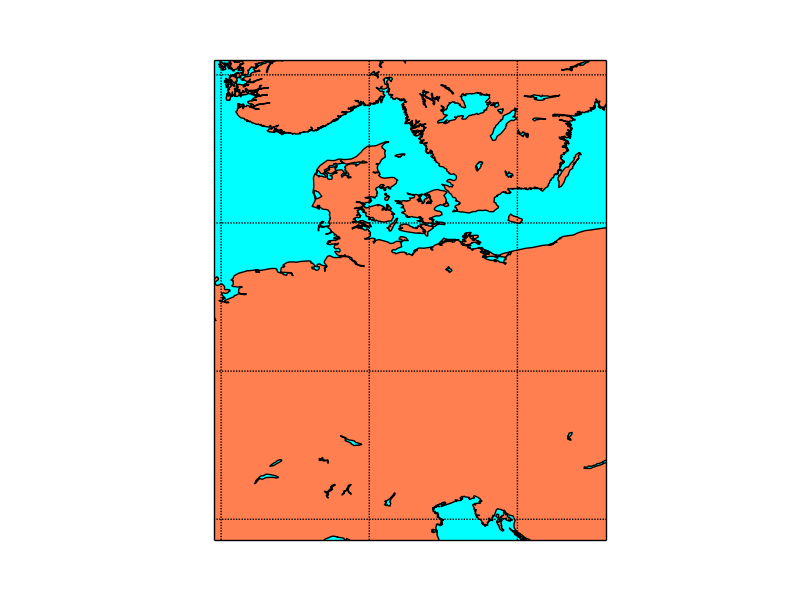
\includegraphics[scale=0.4]{/Users/student/seminar/bsp/bspgrade}
 Mit Beschriftungen:\\
  \lstinputlisting{/Users/student/seminar/bsp/bspgradlabel.py}
  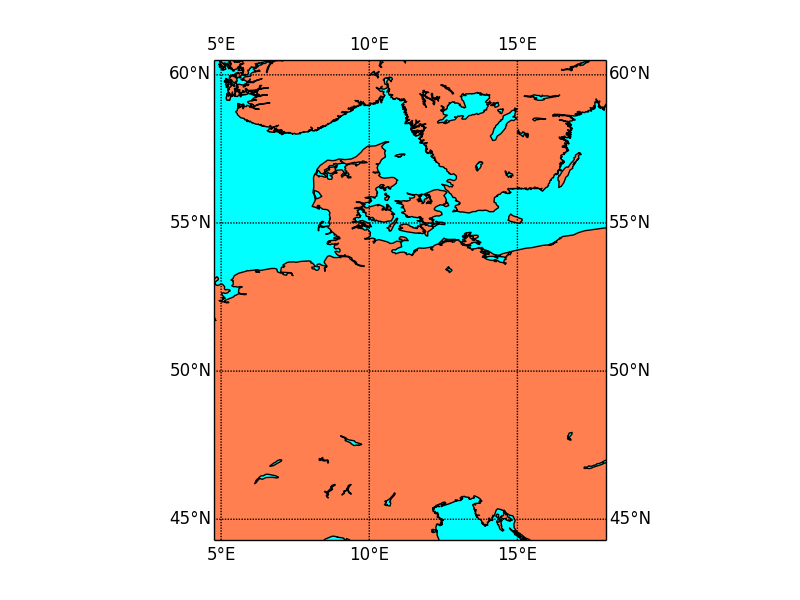
\includegraphics[scale=0.4]{/Users/student/seminar/bsp/bspgradelabel}\newpage 
 \subsubsection*{Maßstab zeichnen}
 Um einen Maßstab zu zeichnen braucht man die Funktion \textsf{drawmapscale(lon, lat, lon0, lat0, length, barstyle='simple', units='km', fontsize=9, yoffset=None, labelstyle='simple', fontcolor='k', fillcolor1='w', fillcolor2='k', ax=None, format='\%d', zorder=None)}. Diese Funktion kann nicht mit der Projektion \textsf{cyl} ausgeführt werden. Die Funktion zeichnet eine Skala an der Position \textsf{lon, lat} der Länge \textsf{length} von dem Punkt \textsf{lon0, lat0}. Die beiden Positionen sind wichtig da die Projektion längenverzerrend sein kann. Man kann den \textsf{barstyle} auf \textsf{fanzy} stellen, dann wird eine Skala gezeichnet bei der sich verschieden farbige Balken abwechseln. Wenn beim Parameter \textsf{labelstyle fancy} angegeben wird, wird über dem Balken noch der Verzerrungsfaktor und die Position \textsf{lon0, lat0} ausgegeben. Mit dem Parameter \textsf{yoffset} kann man die Höhe der Skala und die Entfernung der Beschriftung vom Balken in Metern angeben. Der Defaultwert hierfür ist 2\% der Karten Höhe.\\
 \lstinputlisting{/Users/student/seminar/bsp/bspscalar.py}
 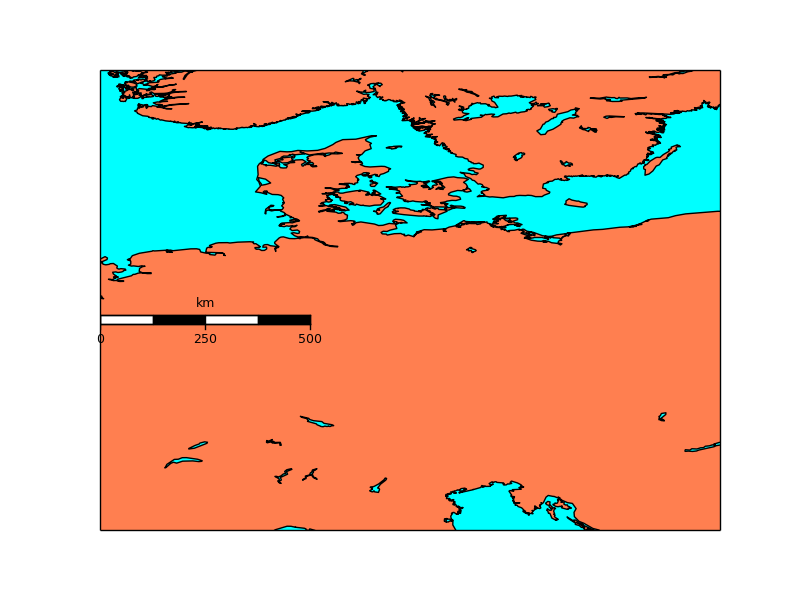
\includegraphics[scale=0.4]{/Users/student/seminar/bsp/bspscalar}\newpage 
 \subsubsection*{Relief zeichnen}
 Um eine Karte mit Relief zu zeichnen kann man die Funktionen \textsf{etopo(ax=None, scale=None, **kwargs)} oder \textsf{shadedrelief(ax=None, scale=None, **kwargs)} benutzen. Die Funktion \textsf{etopo} lädt ein ein Reliefbild von der Seite \textsf{http://www.ngdc.noaa.gov/mgg/global/global.html} als Hintergrund. Die Funktion \textsf{shadedrelief} lädt ein Reliefbild von der Seite \textsf{http://www.shadedrelief.com} als Hintergrund. Mit dem Parameter \textsf{scale} kann man einen Skalierungsfaktor angeben, da die Bilder 10800x5400 groß sind. Was eine gewisse Zeit zum laden und verarbeiten braucht und Speicherplatz verbraucht.\\
 Mit \textsf{shadedrelief()}:\\
 \lstinputlisting{/Users/student/seminar/bsp/bspshadereliev.py}
 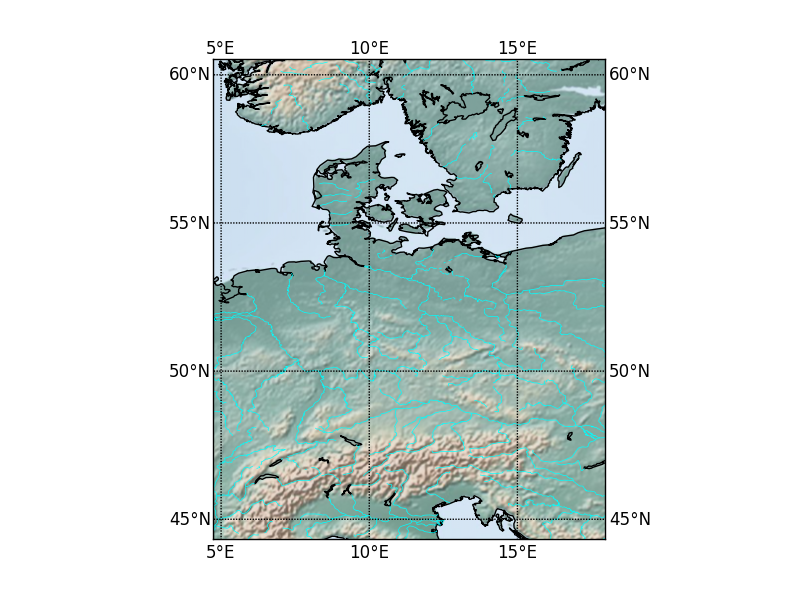
\includegraphics[scale=0.4]{/Users/student/seminar/bsp/bspshadereliev}
 Mit \textsf{etopo()}:\\
 \lstinputlisting{/Users/student/seminar/bsp/bspetopo.py}
 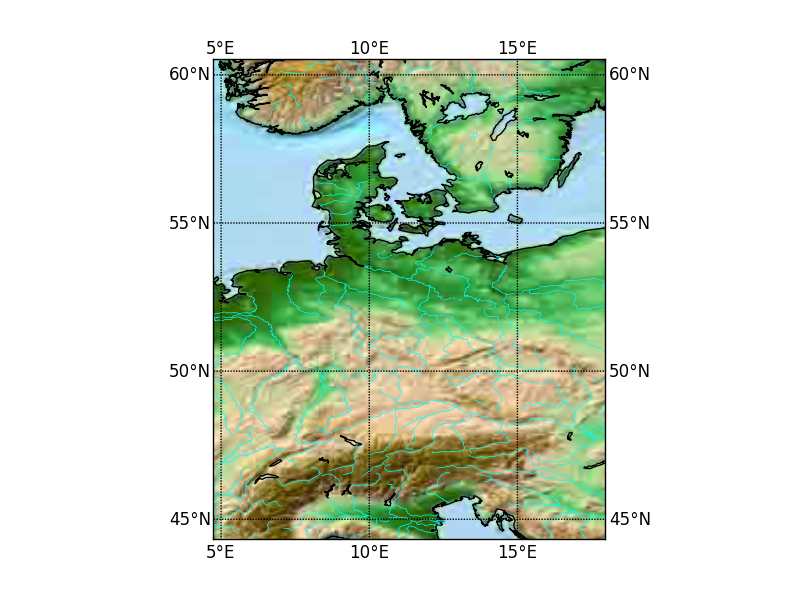
\includegraphics[scale=0.4]{/Users/student/seminar/bsp/bspetopo}
\subsection{Bild auf eine Karte zeichnen}
Um ein Bild auf eine Karte zeichnen zu können, muss das Bild als \textsf{pyplot.image} vorliegen. Dies kann man mit Hilfe der \textsf{PIL} erreichen. Da \textsf{matplotlib.image} eine Funktion \textsf{pil\_to\_array(Pilimage)} zur Verfügung stellt. Beim Zeichnen von Bildern muss man beachten das sie über die ganze Karte gezeichnet werden. Die Funktion um ein Bild zu zeichnen ist \textsf{imshow(X, cmap=None, norm=None, aspect=None, interpolation=None, alpha=None, vmin=None, vmax=None, origin=None, extent=None, shape=None, filternorm=1, filterrad=4.0, imlim=None, resample=None, url=None, hold=None, **kwargs)}. Sie bekommt in \textsf{X} ein Bild als Pixelmatrix übergeben. Die anderen Parameter werden einfach an \textsf{pyplot.imshow()} weitergegeben. Die Parameter \textsf{extent} und \textsf{origin} werden automatisch so gesetzt, das das Bild über die ganze Karte gemalt wird.\\
Mit der Funktion \textsf{warpimage(image='bluemarble', scale=None, **kwargs)} kann man ein Hintergrundbild laden. Dieses Bild muss allerdings den ganzen Globus abdecken. Im Parameter \textsf{image} kann man einen Filenamen oder eine URL angeben. Sollte eine URL angegeben sein wird das Bild von der entsprechenden Seite als temporäre Datei herunter geladen. Dabei muss die URL mit \textsf{http} anfangen. Sollte nichts angegeben sein wird ein \textsf{blue marble next generation} Bild von  
\textsf{http://visibleearth.nasa.gov/} genommen.\\
Mit der Funktion \textsf{wmsimage(server, xpixels=400, ypixels=None, format='png', verbose=False, **kwargs)} kann man ein Hintergrundbild von einem WMS Server laden und zeichnen. Damit diese Funktion funktioniert muss die Karte mit dem passenden Parameter \textsf{epsg} erstellt worden sein, oder die Projektion \textsf{cyl} gewählt sein.\\
Mit der Funktion \textsf{arcgisimage(server='http://server.arcgisonline.com/ArcGIS', service='ESRI\_Imagery\_World\_2D', xpixels=400, ypixels=None, dpi=96, verbose=False, **kwargs)} kann man ein Hintergrundbild von einem ArcGIS Server laden und darstellen. Mit dem Parameter \textsf{service} kann man einstellen welcher Art das Bild sein soll. Um diese Funktion benutzen zu können muss beim erstellen der Karte der Parameter \textsf{epsg} passend gesetzt worden sein, oder die Projektion \textsf{cyl} gewählt sein. Mit den Parametern \textsf{xpixels} und \textsf{ypixels} kann man die Anzahle Pixel in der Breite und Höhe einstellen. Sollte \textsf{ypixels} nicht gesetzt sein wird die Anzahl Pixel in der Höhe von der Anzahl Pixel in der Breite berechnet, so dass das Seitenverhältnis beibehalten bleibt.\\
Mit der Funktion \textsf{bluemarble(ax=None, scale=None, **kwargs)} kann man ein \textsf{blue marbel} Bild als Hintergrund malen. Mit Hilfe des Parameters \textsf{scale} kann man die Pixel Anzahl reduzieren, damit das Bild schneller geladen werden kann. Die Standardgröße des Bildes ist 5400x2700.
\subsection{Daten plotten}
\label{sec:potdata}
Das Module \textsf{Basemap} bietet die Möglichkeit die Plotroutinen von \textsf{pyplot} zu benutzen, da es die Karte mit \textsf{matplotlib} erstellt. Die Karte ist im Grunde ein \textsf{AxesImage}, auf dem dann die entsprechenden Operationen ausgeführt werden. Daher kann man auch die Plotroutinen von \textsf{pyplot} aufrufen da diese ebenfalls mit \textsf{AxesImages} arbeiten. Wenn man mit \textsf{pyplot} zeichnet muss man beachten, dass die Koordinaten, die man angeben muss, in den Projektionskoordinaten der Karte anzugeben sind. Dabei ist die \textsf{Basemap} Klasse sehr hilfreich, sie rechnet nämlich Koordinaten in Längen- und Breitengrad in die Projektionskoordinaten um. Dazu mus man einfach die \textsf{basemap} Instanz mit den Koordinaten als Parameter aufrufen. Dabei können auch mehrere Koordinaten übergeben werden, indem man zwei Felder übergibt.\\
\lstinputlisting{/Users/student/seminar/bsp/bspconvert.py}
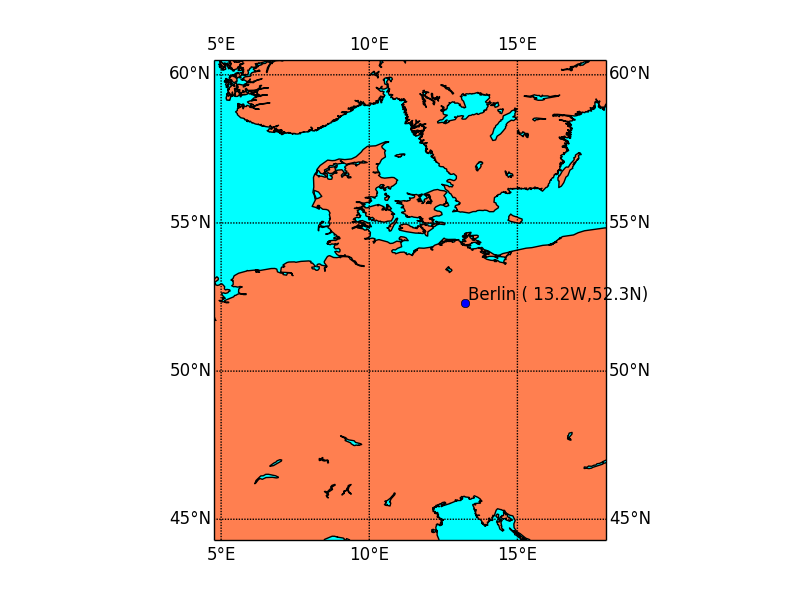
\includegraphics[scale=0.4]{/Users/student/seminar/bsp/bspconvert}\newpage
\subsubsection{Isobaren plotten}
um Isobaren zu plotten braucht man ein zweidimensionales Datenfeld mit den Werten und zwei Felder mit den dazu gehörigen Koordinaten. Diese kann man dann einfach mit Hilfe der Funktion \textsf{contour(x, y, data, *args, **kwargs)} plotten. Die Funktion \textsf{contour} zeichnet Isobarenlinien. Mit der Funktion \textsf{contourf(x, y, data, *args, **kwargs)} werden diese auch gefüllt. Den beiden Funktionen kann man ein \textsf{colormap} Objekt im Parameter \textsf{cmap} übergeben. Dieser Parameter wird dann einfach an \textsf{pyplot} weitergegeben. Darüber kann man den Farbverlauf der Isobaren steuern. Über den Parameter \textsf{levels} kann man angeben welche Wertelevel gezeichnet werden sollen.\\
\lstinputlisting{/Users/student/seminar/bsp/bspcontur.py}
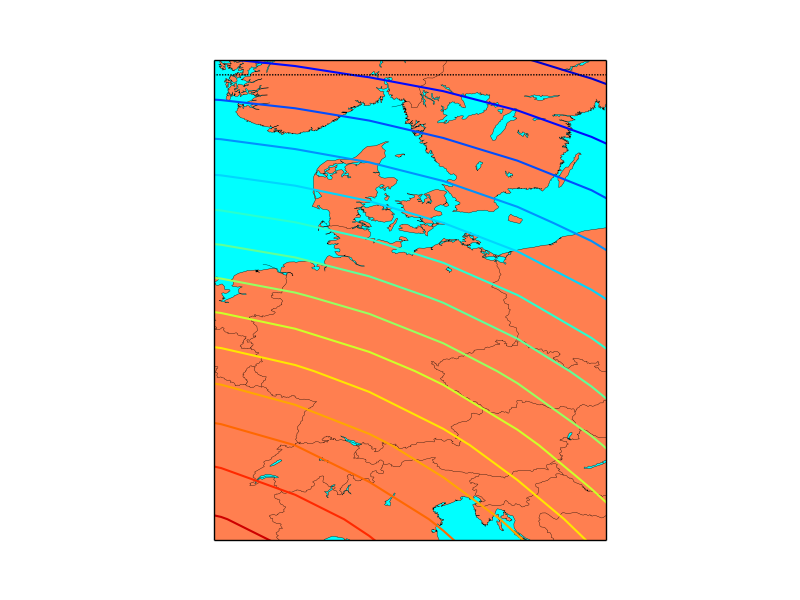
\includegraphics[scale=0.4]{/Users/student/seminar/bsp/bspcont}
Mit der Funktion \textsf{contourf()} muss man aufpassen, dass die Graphik nicht vom Hintergrund übermalt wird. Daher habe ich in dem Beispiel den Kontinent nicht gefüllt.\\
\lstinputlisting{/Users/student/seminar/bsp/bspconturf.py}
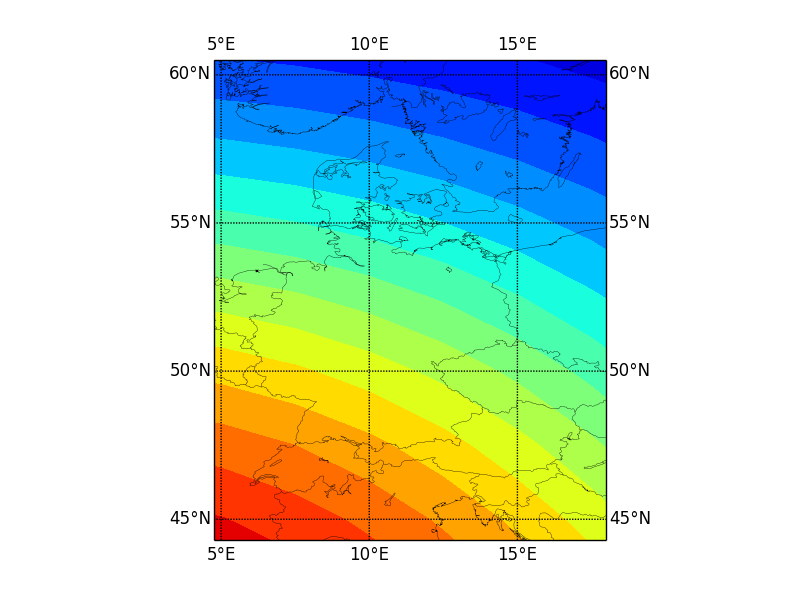
\includegraphics[scale=0.4]{/Users/student/seminar/bsp/bspcontf}\newpage 
\subsubsection{Windmarken plotten}
Mit der Funktion \textsf{barbs(**kw)} kann man einfach Windmarken plotten. Dazu übergibt man der Funktion die Koordinaten der Marke und die Koordinaten des Endpunkts des Vektors der dargestellt werden soll. Die Form der Marke wird durch die Länge des Vektors bestimmt. Eine Flagge bedeutet einen Wert von 50, ein voller Balken 10, ein halber Balken 5. Mit dem Parameter \textsf{barb\_increments} kann man eigene Werte festlegen. Dafür wird dem Parameter ein \textsf{dictionary} mit den \textsf{Schlüsseln} \textsf{half, full, flag} übergeben. Mit dem Parameter \textsf{length} kann man die Länge der Fähnchen in Punkten angeben, der Rest der Marke wird dagegen skaliert.\\
\lstinputlisting{/Users/student/seminar/bsp/bspbarbs.py}
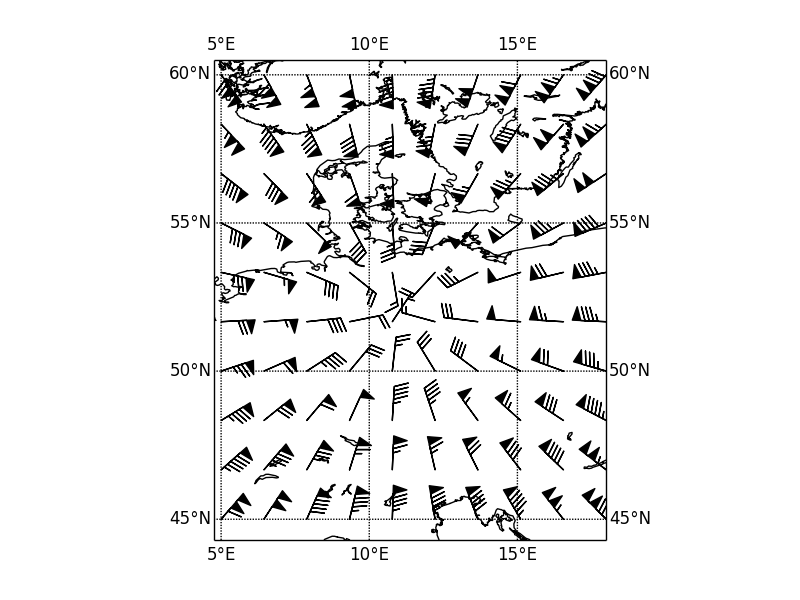
\includegraphics[scale=0.4]{/Users/student/seminar/bsp/bspbarbs}\newpage 
\subsubsection{Windvektoren plotten}
  Mit der Funktion \textsf{quiver(**kw)} kann man Vektoren plotten. Hierbei werden wieder 2 Koordinaten angegeben, wie bei dem Plotten von Windmarken. Mit den Parametern \textsf{u,v} wird ein Vektor übergeben der gezeichnet werden soll. Mit den Parametern \textsf{scale, scale\_units} kann man bestimmen wie lang die Vektoren werden. Je kleiner der \textsf{scale} Parameter desto größer wird der Vektor. Wenn man bei diesen Parametern nichts angibt wird der Wert automatisch aus den zu zeichnenden Vektoren ermittelt.\\
  \lstinputlisting{/Users/student/seminar/bsp/bspquiver.py}
  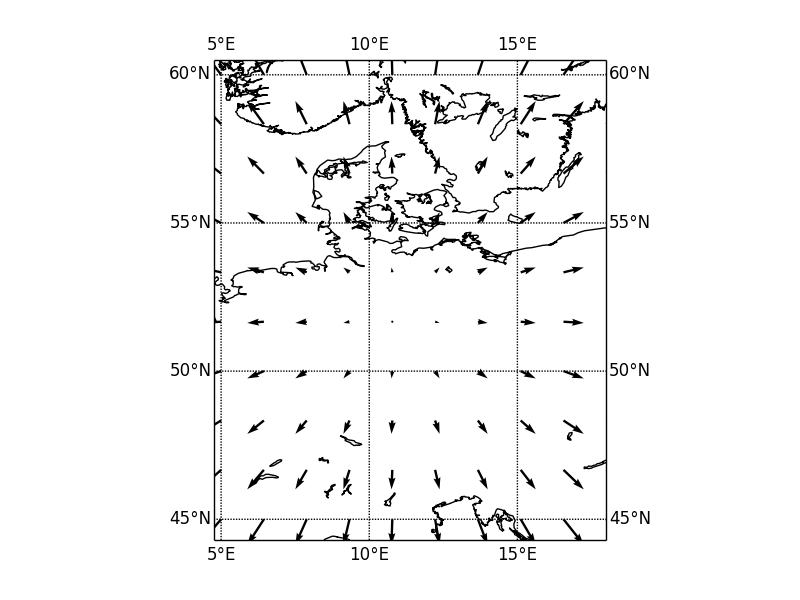
\includegraphics[scale=0.4]{/Users/student/seminar/bsp/bspquiver}\newpage 
  \subsubsection{gekrümmte Strecken plotten}
  Um Strecken wie zum Beispiel eine Flugroute von New York nach London zu plotten, benutzt man am Einfachsten die Funktion \textsf{drawgreatcircle(lon1, lat1, lon2, lat2, del\_s=100.0, **kwargs)}. Diese Funktion zeichnet einen Bogen von den Koordinaten \textsf{lon1,lat1} nach \textsf{lon2,lat2} dabei werden Punkte alle \textsf{del\_s} km ermittelt. Diese Punkte kann man sich auch mit der Funktion \textsf{gcpoints(lon1, lat1, lon2, lat2, points)} berechnen lassen.\\
  \lstinputlisting{/Users/student/seminar/bsp/bspgreatcirc.py}
  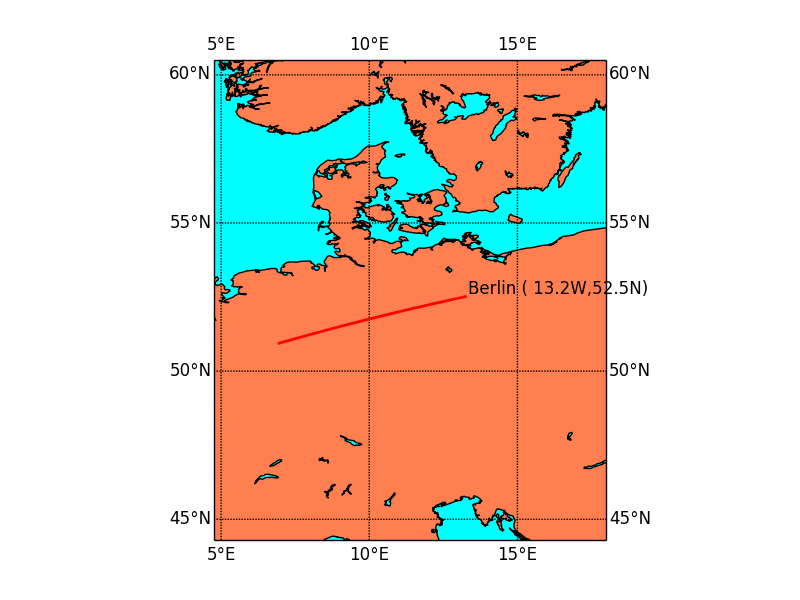
\includegraphics[scale=0.4]{/Users/student/seminar/bsp/bspgreatcirc}\newpage 
  \subsubsection{Viele Punkte plotten}
  Mit der Funktion \textsf{scatter(x, y, s=20, c=u'b', marker=u'o', cmap=None, norm=None, vmin=None, vmax=None, alpha=None, linewidths=None, verts=None, hold=None, **kwargs)} kann man Marken plotten. Diese werden an die Positionen die durch \textsf{x,y} definiert sind gezeichnet. der Parameter \textsf{s} gibt die Größe der Marke an. Der Parameter \textsf{marker} gibt an was für eine Marke gezeichnet werden soll. Über den Parameter \textsf{c} kann man die Farben der Marken bestimmen.
  \lstinputlisting{/Users/student/seminar/bsp/bspscatter.py}
  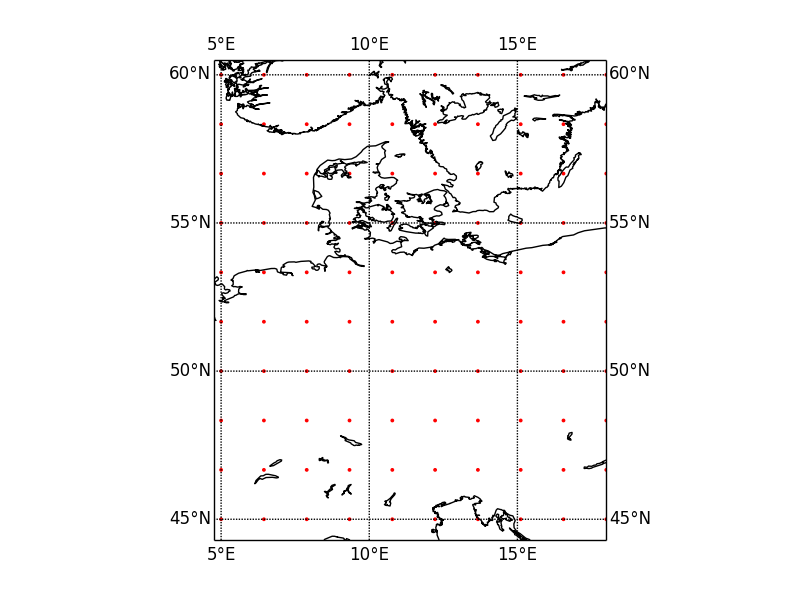
\includegraphics[scale=0.4]{/Users/student/seminar/bsp/bspscatter}\newpage 
   \subsubsection{Linienzüge zeichnen}
   Linienzüge lassen sich mit der Funktion \textsf{plot(x,y,**kw)} zeichnen. Diese Funktion zeichnet einen Linie von einem Punkt zum Nächsten. Dabei kann man \textsf{x,y} einfach als Felder übergeben. Hierbei ist zu beachten das davon ausgegangen wird das die Koordinaten Projektionskoordinaten sind.
\subsection{Karte speichern}
\label{sec:save}
Um die Karte die man erstellt hat zu speichern bedient man sich des Moduls \textsf{pyplot}. Von diesem Modul kann man die Funktion \textsf{savefig(fname, dpi=None, facecolor='w', edgecolor='w', orientation='portrait', papertype=None, format=None, transparent=False, bbox\_inches=None, pad\_inches=0.1, frameon=None)} benutzen um die Figur zu speichern. Dazu gehören auch die Farblegende und der Titel der Figur. Es wird also nicht nur die Karte gespeichert. Mit dem Parameter \textsf{fname} wird der Dateiname angegeben in den gespeichert werden soll. Mit dem Parameter \textsf{format} kann ein unterstütztes Format angegeben werden, diese können variieren, meistens werden die Formate \textsf{png, pdf, ps, eps, svg} unterstützt. Die Parameter \textsf{papertype} und \textsf{orientation} werden eventuell nur für das \textsf{ps} Format unterstützt.
\subsection{Karte anzeigen}
\label{sec:show}
Mit der \textsf{pyplot} Funktion \textsf{show()} kann man die Karte anzeigen lassen. In der Anzeige kann man dann auch zoomen und die Karte verschieben. Was es einem ermöglicht auch Zeichnungen außerhalb der eigentlichen Karte zu sehen.\newpage
\subsection*{Literatur}

http://matplotlib.org/basemap
Basemap Dokumentation.\newpage
\section*{Nomenklatur}
\subsection*{$\calR$}
Der Radius der Erde.
\subsection*{$\varphi$}
Der Breitengrad der Polarkoordinate.
\subsection*{$\lambda$}
Der Längengrad der Polarkoordinate.
\subsection*{&\calX&}
Die X Koordinate der 2D Projektion.
\subsection*{&\calY&}
Die Y Koordinate der 2D Projektion.\newpage
\section*{Glossar}
\subsection*{Flächentreu}
Flächentreu heißt, dass der Maßstab mit dem Flächen verkleinert werden auf der gesamten Karte gleich ist. Dies führt an den Rändern zu Verzerrungen.\newpage
\end{document}
